\section{Are parasites a selective force in the European house mouse hybrid zone?}
\subsection{Hybrids are not an average of their parents}
Species can be defined as groups of interbreeding natural populations that are reproductively isolated from each other (“biological species concept” proposed by \cite{mayr_animal_1963}). Hybrids appear when two species, or more largely two genetically distinct populations, meet and reproduce \citep{barton_analysis_1985}. Artificial animal hybridisation may be almost as old as selective animal breeding itself. The oldest known example is the mule, hybrid of a female horse and a male donkey, especially enduring, able to transport heavy burden, but sterile \citep{leighton_mule_1967}. 
\par
Hybrids can be superior than both parental populations for specific traits such as size, strength and growth. This phenomenon, called \textbf{heterosis} or \textbf{hybrid vigour}, is especially pronounced when parents come from two inbred populations \citep{brenner_heterosis_2001}. Hybrid vigour is maximum in the first generation of crossing, F1, where heterozygosity is at its highest. The \textbf{dominance hypothesis} states that the increase of heterozygosity in hybrids leads to the purge of deleterious recessive mutations in homozygous. According to the \textbf{overdominance hypothesis}, heterozygosity at one locus can even improve some traits compared to parents \citep{crow_overdominance_2001}. Overdominance is for example one of the possible explanations for the maintenance of high levels of genetic diversity of Major Histocompatibility Complex (MHC, set of genes coding for proteins involved in vertebrate immunity) \citep{read_major_2001, sommer_importance_2005}. Finally, interaction between genes could participate in hybrid vigour \parencite[\textbf{positive epistasis};][]{schnell_multiplicative_1992}, as was shown for the growth of the well-studied plant model, \textit{Arabidopsis thaliana} \citep{vanhaeren_combining_2014}.
\par
However, hybridisation does not necessarily result in hybrid superiority for all phenotypic traits. The heterozygous advantage can be counteracted by \textbf{genetic incompatibilities}. Firstly described by Bateson in the early 20th century \citep{bateson_heredity_1909}, these incompatibilities arise from the admixture of (at least) two alleles that have never before coexisted, and therefore create deleterious effects when brought together from distinct populations \citep{dobzhansky_studies_1936, muller_isolating_1942, orr_population_1995}. Later work on \textit{Drosophila} hybrids showed that these incompatibilities commonly involve three genes or more \citep{cabot_genetics_1994, palopoli_genetics_1994}, and interactions between genes \parencite[\textbf{negative epistasis};][]{larson_evolution_2018}. Hybrid incompatibilities can affect hybrid relative \textbf{fitness}, i.e. its reproductive success compared to other genotypes of the same population, in this case the parental genotypes \citep{krimbas_fitness_2001}. Total or partial \textbf{hybrid inviability} or \textbf{hybrid sterility} can act as reproductive barrier between two genetically distinct populations \citep{coyne_reproductive_2001}. In case of fertility decrease, Haldane first described that the heterogametic sex is the one more likely to be affected \citep{haldane_sex_1922}. Moreover, some \textbf{speciation genes} \parencite[genes underlying reproductive isolation;][]{wu_genes_2004} have been identified, mainly in \textit{Drosophila} genus \citep{oliver_accelerated_2009}. The \textit{prdm9} gene identified in mice is so far the only vertebrate gene known to participate in hybrid male sterility \citep{mihola_mouse_2009}. 
\par
Traditionally, hybrids were thought of as a rarity, but it seems now that a large proportion of plants (10\%) and animals (25\%) can produce hybrids in nature \citep{mallet_hybridization_2005}. Not only studying hybrids allows us to understand the mechanisms of speciation, but hybridisation with introduced species can threaten autochthonous endangered animals, making studies of hybridisation relevant for conservation biology \citep{simberloff_hybridization_1996}. \cite{stronen_perspectives_2013} also argue that the specific ecological role of hybrids could justify their protection by conservation policies. Moreover, hybrid zones represent melting pots of genotypes that allow to explore the impact of genetic diversity on several physiological systems (e.g. reproduction, immunity).
\par
In this thesis, we focus on a well studied system, the European house mouse hybrid zone (HMHZ).

\subsection{The European house mouse hybrid zone, a tension zone}
The house mouse (\textit{Mus musculus}) is the most widely used animal model in biomedicine. However, the vast majority of inbred lines used nowadays are not “natural” animals: they originate from pet mice from the late 19th and beginning of 20th century, and are mixtures of four different subspecies \citep{davisson_chapter_2004}. The common ancestor to all \textit{Mus musculus} subspecies originates from the Indo-Pakistani cradle. Several subspecies emerged after expansion from this cradle, commensal mice following human migrations \citep{boursot_evolution_1993}. At least five subspecies have been described based on phylogenetic analysis: \textit{M. m. musculus}, \textit{M. m. domesticus}, \textit{M. m. castaneus}, \textit{M. m. molossinus}, and \textit{M. m. gentilulus}. There is a wide range of evidence that these subspecies are not in complete reproductive isolation, and that gene flow can occur between them in zones of secondary contact \citep{auffray_house_2012}. In Europe, \textit{M. m. domesticus} (hereafter Mmd) and \textit{M. m. musculus} (hereafter Mmm) entered into secondary contact around the Bronze Age after having taken different colonisation routes, respectively south and north of the Black Sea, and, thus, diverging (mostly) in allopatry for about half a million years \citep{duvaux_isolation_2011, geraldes_inferring_2008, geraldes_higher_2011}. This secondary contact formed a belt of about 20 km wide and more than 2500 km long, running from Denmark to the Black Sea: the European house mouse hybrid zone (hereafter HMHZ) \citep{baird_what_2012, boursot_evolution_1993}(\textbf{Figure 1.1}). Despite the fact that they can form hybrids, these two subspecies differ in several traits including pelage color, tail/body length ratio (shorter for Mmm than for Mmd) \citep{boursot_evolution_1993}, boldness and activity \citep{frynta_behavioural_2018}, and male aggressiveness \citep{dureje_no_2010}.

\begin{figure}[H]
    \centering
    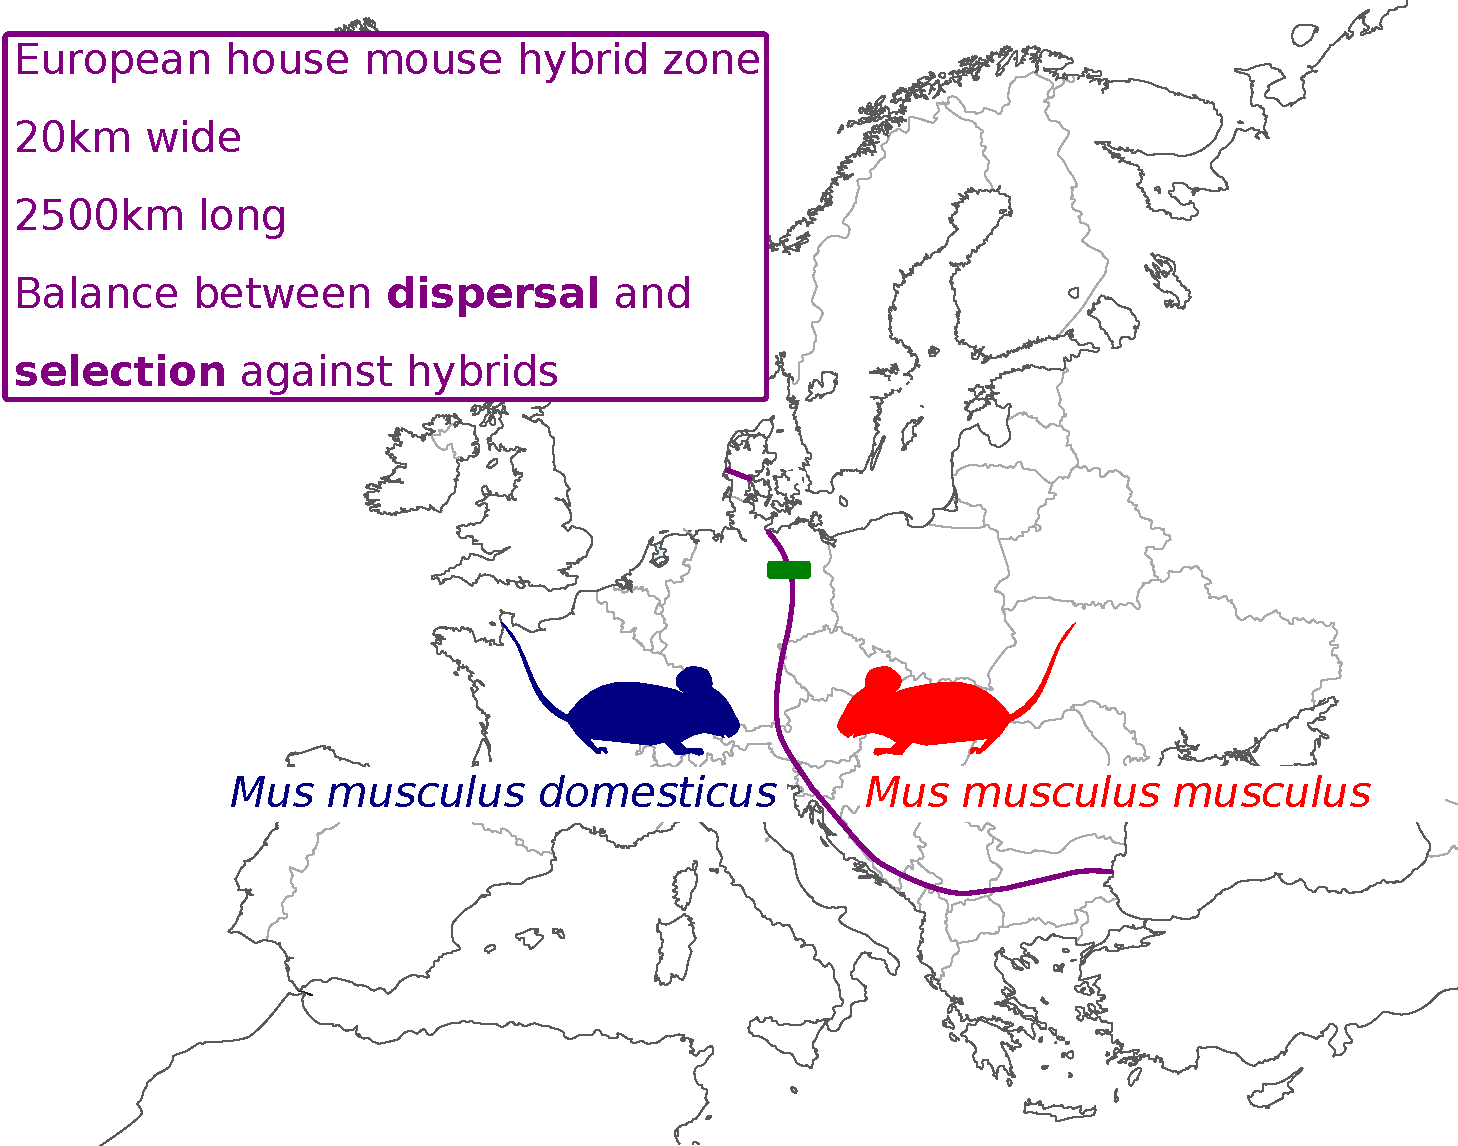
\includegraphics[width=.7\linewidth,height=\textheight,keepaspectratio]{images/1introduction/Figure1.pdf}
    \caption{Approximate course of the European house mouse hybrid zone (purple line) between \textit{Mus musculus domesticus} (blue) and \textit{Mus musculus musculus} (red) areas. (adapted from \cite{baird_where_2012}. Green square: Heitlinger group transect.}
\end{figure}

Through the HMHZ, the gene flow between both subspecies is not completely interrupted, and introgression of genes from one side to the other happens \citep{macholan_genetic_2007, macholan_assessing_2011, macholan_widespread_2019, raufaste_inferences_2005}. Hybrids between Mmd and Mmm are highly recombinant, presenting a range of genotypes, and no F1 or early-generation hybrids have been found \citep{macholan_genetic_2007}. Numerous genetic studies performed over geographically independent transects of the HMHZ \parencite[e.g.][]{macholan_genetic_2007, payseur_differential_2004, raufaste_inferences_2005} give strong support to the \textbf{tension zone} model in this system: the immigration of less hybridised mice to the centre of the zone, increasing the hybrid population size, is balanced by endogenous selection against hybrids \citep{baird_what_2012, barton_analysis_1985, boursot_evolution_1993}. This negative selection of hybrids seem to be linked with sterility or fertility \citep{baird_what_2012} and disruption of their spermatogenesis has been shown \citep{albrechtova_sperm-related_2012, martincova_sperm_2019, turner_reduced_2012, turner_genome-wide_2014}.
\par
Additionally, interaction with parasites (in this thesis, we will use the term “parasite” in the restricted eukaryotic sense, unless stated otherwise) has long been suggested to participate in the maintenance of the HMHZ. The next section will describe the long-lasting controversy around this issue.

\subsection{Parasites as hosts’ selective factor}
Parasites are ubiquitous in natural systems and affect human and animal health alike \citep{schurer_community-based_2016}. Their close interaction with their hosts over several generations and incentive to develop tactics to escape the host immune system led to consider parasites as plausible selective force for their hosts \citep{schmid-hempel_parasitesnew_2009}. There is evidence that parasites can manipulate vertebrate hosts behaviour, including the part related with reproduction \citep{klein_parasite_2003}. They can also affect their host community structure as was shown empirically in macroinvertebrates of New Zealand, where nematode density on cockles affect the full intertidal community \citep{mouritsen_parasites_2005}. It stands to reason that parasitic infections have been hypothesised to be a potential driving factor of maintenance or break-up of species barriers in hybrid zones \citep{sage_wormy_1986} (\textbf{Figure 1.2}).

\begin{figure}[H]
    \centering
     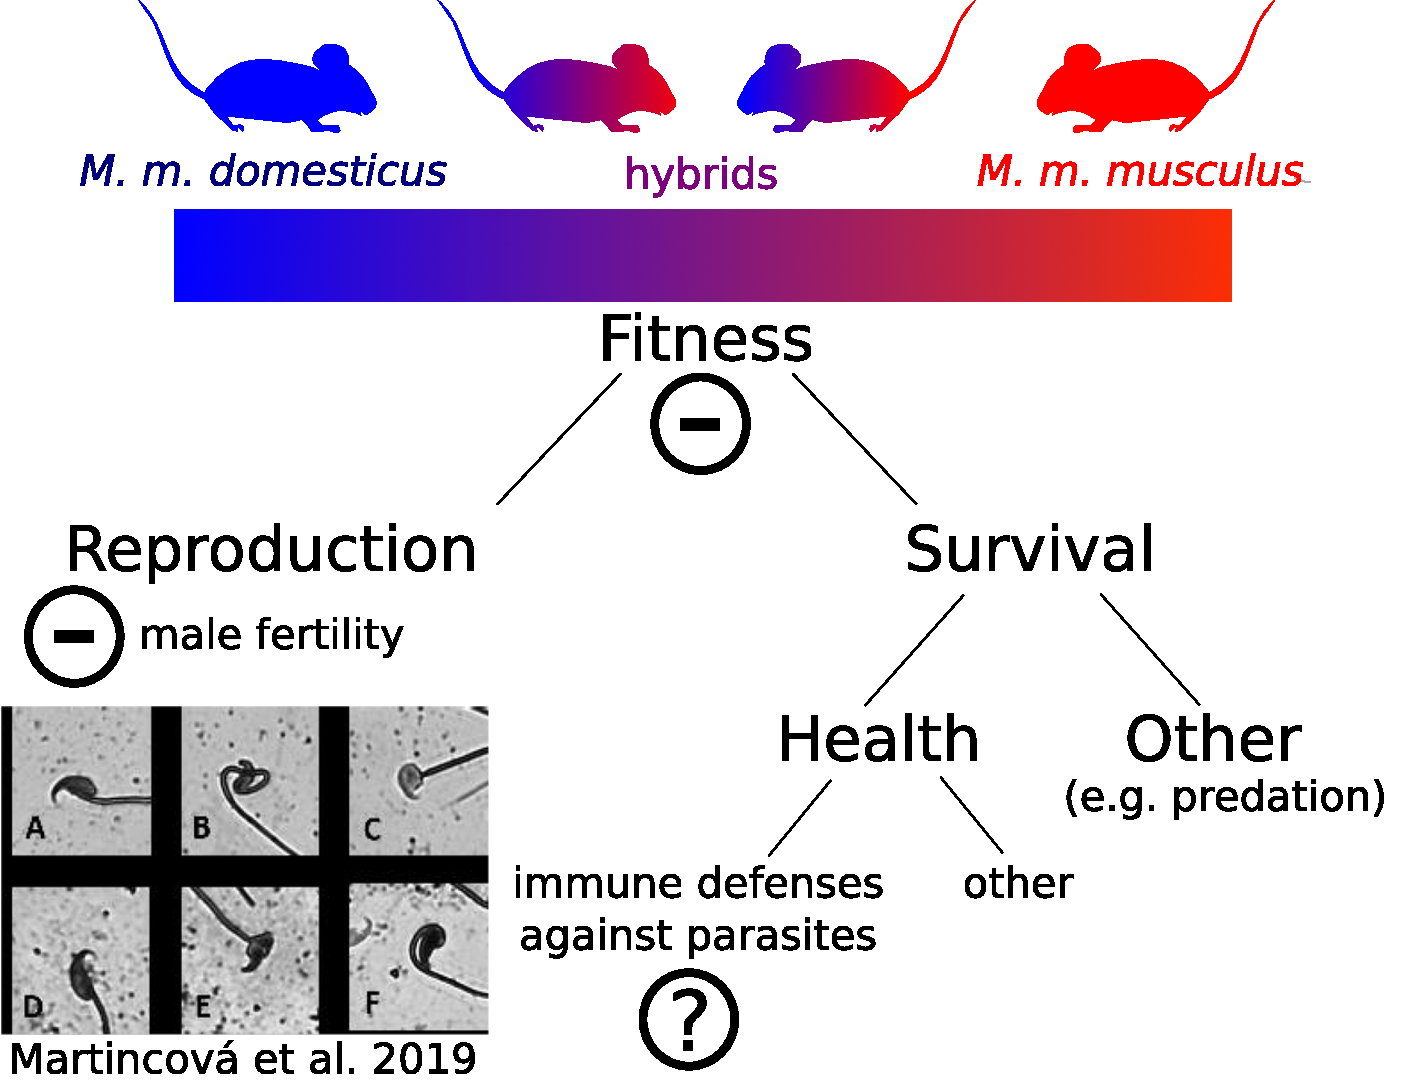
\includegraphics[width=.7\linewidth,height=\textheight,keepaspectratio]{images/1introduction/Figure2.pdf}
    \caption{\textbf{Hybrid fitness is reduced in the HMHZ} \citep{baird_what_2012}. Reproduction is negatively affected in hybrids, mainly via disruption of spermatogenesis (photography: various sperm heads from F1 experimentally produced hybrids. Figures A \& D: normal sperm heads; Figures B, C and E, F: abnormal sperm heads \parencite[source:][]{martincova_sperm_2019}. How hybrid health is affected by parasites is a long lasting debate.}
\end{figure}

The HMHZ is the first animal hybrid zone studied for differences in parasite loads \citep{sage_wormy_1986}. Original results seemed to indicate elevated worm load in hybrids. This was interpreted as hybrid incompatibilities: after having evolved separately within each subspecies, coadapted gene complexes in the immune system would be broken down in hybrids, which would lead to fitness reduction \citep{moulia_wormy_1991, moulia_experimental_1993, sage_wormy_1986}. However, further infection studies showed inconsistencies. Hybrids showed higher parasite loads compared to parents with the protozoan \textit{Sarcocystis muris} \citep{derothe_susceptibility_2001}, but reduced parasite loads (i.e. hybrid vigour on resistance) not only in F1 \citep{moulia_hybrid_1995} but also in later recombinant crossings F3 and F4 \citep{derothe_recombination_2004} following laboratory infection with helminths. More recently, a field study confirmed that hybrids had reduced helminth loads compared to parentals \citep{baird_where_2012}.
\par
All these different studies disagree on two major points: (1) the direction of hybrid effect of parasitism (are hybrids more resistant or more susceptible to parasites?) and (2) the role of parasites as selective factor. Indeed, to fully understand the possible impact of parasites on animals in the HMHZ, one must answer this question: does a change in parasite load necessarily imply a change in fitness? Before making assumptions on the impact of parasites on host fitness, there is a need to explore more thoroughly the different defense mechanisms of mice against parasites.

\section{Host immune defenses against parasites}
\subsection{Resistance and tolerance}

Parasites are by definition harmful to their hosts, and therefore imply costs \citep{noauthor_parasitism_2019}. These can be direct, including tissue damages and drain of host nutrients, or indirect, for instance, the decline of body condition that can lead to higher susceptibility to further infections \citep{beldomenico_poor_2008}, or by increasing susceptibility to predation \citep{bakker_parasite-induced_1997, ostlund-nilsson_parasitic_2005}. Hosts can defend themselves against parasitic infections in numerous ways. The first line of protection is provided by avoidance of parasites. If this strategy fails and the host gets infected, then the host immune system steps in \citep{schmid-hempel_evolutionary_2013}. \textbf{Resistance} is the ability of a host to reduce its pathogen burden. It results from host defense against infection or proliferation \citep{raaberg_decomposing_2009}. Resistance reduces parasite fitness by definition. However, when the immune response targeted at the parasite causes disease to the host (\textbf{immunopathology}), resistance can reduce host fitness too \citep{graham_evolutionary_2005}. 
\par
To deal with both the direct damages created by parasite infection and immunopathology, a second line of defense comes into play. \textbf{Disease tolerance} (not to be confused with immune tolerance which is the unresponsiveness of an immune system to a pathogen) is the ability of a host to reduce the damage induced by a certain parasite burden \citep{raaberg_decomposing_2009}, on health (\textbf{mortality tolerance}) or more indirectly on fecundity (\textbf{sterility tolerance}) \citep{best_maintenance_2008}. It is usually measured as the slope of a fitness trait, often a health measurement supposed to alter fitness eventually (e.g. body weight), on parasite load. It can be calculated in two ways: \textbf{range tolerance} measures a reaction norm, i.e. a change of phenotypic expression of the fitness trait in one genotype across a range of environments (in this case, several parasite loads). \textbf{Point tolerance} instead measures health at one single parasite load. These two measures can possibly give different results when different hosts present different health conditions when not infected with parasites, or when the relationship between health and parasite load is not linear \citep{little_coevolution_2010}. This can be problematic for field studies, where host health for a null parasite load and health-parasite load relationship are usually unknown, as confounding factors (e.g. coinfections, age, lactation status) come into play. Tolerance by definition increases the overall host fitness for a particular parasite load. Contrary to resistance, tolerance also increases parasite fitness, e.g. by providing parasite with a longer living niche, the host \citep{kutzer_maximising_2016, miller_evolution_2006, roy_evolutionary_2000}. 
\par
Resistance and tolerance are costly: in order to defend themselves against parasites, hosts consume resources that could have otherwise been used for other physiological functions \citep{sheldon_ecological_1996}. In the next section, we will examine the nature of the costs of defense mechanisms for the hosts. For the sake of conciseness, unless otherwise stated, we will focus on vertebrate hosts.

\subsection{Immune defenses are costly}
Resistance can result from a large range of mechanisms, from simple presence of unspecific biological barriers, to limitation of specific parasite growth. For the latter, the activation of innate and adaptive immune arms of the immune system comes with an energetic cost to the host \citep{schmid-hempel_evolutionary_2013}. This cost is typically measured by associating individual parasite load with fitness-associated functions. For example, resistance to parasites measured as (inverse of) fecal egg counts is reduced in lactating females in several animals including bighorn ewes \citep{festa-bianchet_individual_1989} and spotted hyena \citep{east_does_2015}. Lactation is a critical life-history stage for the survival of offspring and resource-demanding to the mother, hence it is hypothesised to be prioritised over maximum resistance to parasites.
\par
After establishment of infection, several mechanisms enter in action to increase tolerance, without targeting parasite growth, but rather the consequences of infection on host fitness. These mechanisms, much less studied than resistance mechanisms, mainly consist in protection from tissue damage or from alteration of host physiology, caused by pathogens or by the immune response \citep{medzhitov_disease_2012}. For example, \cite{reece_innate_2006} have showed that mice lungs inflammation induced by infection with the hookworm \textit{Nippostrongylus brasiliensis} is reduced by the induction of alternatively activated alveolar macrophages. In another rodent, field voles, \cite{jackson_immunological_2014} identified a mediator of Th2 immunity (the transcription factor Gata3) as tolerance marker, improving body condition and survival upon infection with macroparasites in mature animals. In this system, Gata3 was also negatively correlated with testis weight, suggesting a cost of tolerance in terms of reproductive effort.
\par
The optimal level of both defense mechanisms is determined by the balance between costs associated with parasitism, with resistance and with tolerance \citep{sheldon_ecological_1996}. Theory predicts that resistance alleles should present polymorphisms maintained by balancing selection, while tolerance alleles should evolve to fixation \citep{roy_evolutionary_2000, miller_evolution_2006}. Nevertheless, empirical studies do not all detect such pattern. Laboratory mouse strains infected with \textit{Plasmodium chabaudi} \citep{raaberg_disentangling_2007} present a negative correlation between resistance and tolerance (a given strain presenting intermediate levels of resistance and tolerance, high resistance and low tolerance, or vice versa). Similar results were found in infection of sea trout (\textit{Salmo trutta trutta}) and Atlantic salmon (\textit{Salmo salar}) with the trematode \textit{Diplostomum pseudospathaceum} \citep{klemme_vertebrate_2016}. This could be due to the redundancy of resistance and tolerance, resulting in trade-offs \citep{restif_concurrent_2004, fornoni_evolution_2004}. 
\par
\cite{kutzer_maximising_2016} noted that if studies addressing resistance are common, those addressing tolerance are more scarce. They suggest increasing the number of longitudinal studies and note that a host-centric view of tolerance is unsatisfactory, as host fitness also depends on the parasite \textbf{virulence}. In its strict sense, virulence means host mortality rate caused by parasite infection \citep{anderson_coevolution_1982}; in a more general sense evolutionary biologists sometimes use it as reduction of host fitness (health or fecundity) upon infection \citep{little_coevolution_2010}. For the reasons above developed, studying jointly resistance and tolerance is necessary to correctly assess the impact of parasites on their hosts. Importantly, this requires suitable host-parasite models, possibly with various levels of virulence in the same host.

\section{Our parasite model: \textit{Eimeria} spp.}
\subsection{\textit{Eimeria} spp. trigger a Th1 immune response}
We have seen earlier (1.3.) that the majority of studies (and all of the field studies) investigating the role of parasitism in the maintenance or break-down of species barrier in the European house mouse hybrid zone focused on helminths. As extracellular macroparasite, they trigger mainly a T helper type 2 (Th2) immune response \citep{sher_regulation_1992}. The effect of hybridization in terms of immune defenses of hybrid mice against parasites relatively to parental mice (higher, lower, or average) could depend on the type of immune response triggered. For this reason, we chose to focus our work on an intracellular microparasite genus, triggering a T helper type 1 (Th1)-mediated response \citep{sher_regulation_1992}, \textit{Eimeria}. In our second Chapter, we considered also helminths (more precisely pinworms) for comparison.
\par
The \textit{Eimeria} genus belongs to the phylum of Apicomplexan protozoan parasites. Their host range is extremely wide and includes birds, mammals, reptiles, amphibians and fish \citep{chapman_chapter_2013}. They are described particularly well in domestic animals due to their economical importance, especially in poultry \citep{blake_securing_2014}, but can also be found in wild animals, where they are potentially problematic for conservation \parencite{jeanes_two_2013, knowles_stability_2013, matsubayashi_molecular_2018}. Each of the >1800 described \textit{Eimeria} species is generally considered strictly host specific \citep{duszynski_eimeria_2011}, but the recent use of multilocus genetic markers method in rodents showed that this host specificity could be less strict than previously thought \citep{jarquin-diaz_generalist_2020}. \textit{Eimeria} oocysts, the infectious stage, are released in the environment via the feces and infect the next host by oral-fecal contamination. The parasites infect epithelial digestive cells of their hosts, which leads to malabsorption of nutrients and weight loss. The \textit{Eimeria} life cycle presents both asexual (schizogony) and sexual (gametogony) phases, and takes place in a single host \citep{burrell_life_2019}.
\par
\textit{E.~falciformis} is the gold standard for murine \textit{Eimeria} research. Host defense mechanisms against this parasite are well studied \parencite[see for example][]{mesfin_pathological_1978, pogonka_cd8_2010, schmid_apicomplexan_2012} and its whole genome is sequenced and annotated \citep{heitlinger_genome_2014}. T-cells have been shown to play a major role in the defense against \textit{E.~falciformis} infection \citep{mesfin_thymic_1979, stiff_effect_1990}. Following infection, interferon γ (IFNγ) is upregulated \citep{schmid_eimeria_2014}, and experimental infections showed higher weight loss and pathology but lower oocysts shedding in IFNγ-deficient mice than in wild type \citep{stange_il-22_2012}. IFNγ could in this respect be seen as a tolerance factor. \cite{ehret_dual_2017} compared host and \textit{E.~falciformis} transcriptomes (dual transcriptomes) in immunocompetent and immunodeficient laboratory mice, and in naïve and challenged laboratory mice. They did not find differences in the gene expression profile of this parasite between hosts, and concluded that \textit{E.~falciformis} does not respond plastically to the host environment but rather present a genetically canalised (“hard wired”) program of infection. 
\par
By considering \textit{Eimeria} spp. and helminths jointly, triggering Th1 and Th2 immune responses, we attempted to assess the generality of hybrid response in nature (\textbf{Chapter 1}). On a note of caution, in the field, one can only assess the impact of parasite species that are prevalent enough to allow robustness of statistical tests. Using a complementary laboratory approach can solve this issue (\textbf{Chapter 2}).
\subsection{Focus on two \textit{Eimeria} species: \textit{E.~falciformis} and \textit{E.~ferrisi}}
In a recent study performed by our group in the HMHZ, three \textit{Eimeria} species have been identified: \textit{E.~ferrisi}, \textit{E.~falciformis}, and \textit{E. vermiformis} with prevalences of 16.7\%, 4.2\% and 1.9\%, respectively \citep{jarquin-diaz_detection_2019}. Current markers were not able to detect a population structure for \textit{Eimeria} spp. in the HMHZ \citep{jarquin-diaz_generalist_2020}. The two most prevalent \textit{Eimeria} species, \textit{E.~ferrisi} and \textit{E.~falciformis}, present close ecological niches \parencite[\textit{E.~ferrisi} infects the cecum villar epithelial cells and \textit{E.~falciformis} the cecum crypt cells;][]{schito_comparison_1996}, but different virulence in laboratory mice. More precisely, the life cycle of \textit{E.~ferrisi} is shorter than that of \textit{E.~falciformis} \citep{al-khlifeh_eimeria_2019, schito_comparison_1996}. They both provoke similar symptoms in laboratory mice, mainly diarrhea, lesion of the enteric epithelium, and weight loss \citep{ankrom_life_1975, ehret_dual_2017, schito_comparison_1996}. In a study using the laboratory Swiss mouse strain, \cite{tilahun_oocyst_1981} found a higher mortality rate for \textit{E.~ferrisi} (2 out of 5 mice died when infected with 10$^5$  oocysts) than for \textit{E.~falciformis} (no death observed for the same inoculum). Though, they note that a former study described another isolate of \textit{E.~falciformis} far more lethal, killing mice from an inoculum of 2000 oocysts \citep{mesfin_pathological_1978}. More recently, using a lower infective dose (200 oocysts) on the laboratory NMRI mouse strain, we observed a stronger virulence of two different isolates of \textit{E.~falciformis} compared with one of \textit{E.~ferrisi}, both in terms of weight loss and mortality, correlated with a stronger immunopathology \citep{al-khlifeh_eimeria_2019}. The observed discrepancies in these in vivo experiments can be due to potential attenuation of virulence in case oocysts are collected early in the infection cycle \citep{mcdonald_endogenous_1987}, to modified virulence of specific parasite isolate over time in the lab, or to different immune systems of each mouse strain. \textit{E.~ferrisi} has been less intensively studied than \textit{E.~falciformis}; nevertheless, mortality after infection and oocysts output were found to differ between eight tested laboratory mouse strains, and T-cells also play a role in resistance to this parasite \citep{klesius_strain-dependent_1979}.
\subsection{Proxies for resistance and tolerance to \textit{Eimeria} spp.}
Resistance against murine \textit{Eimeria} species can be estimated by the inverse of parasite load. In our field study (\textbf{Chapter 2}), \textit{Eimeria} load was measured by the quantity of parasite gene in the infected tissues (ileum and caecum) per mouse gene. We also assessed the impact of infection on host health: body condition was calculated as individual residuals from ordinary least-squares regression of body weight by body length (separately for males and females). of note, this is not an estimation of tolerance, as individual weight before infection cannot be known in the field (apart from capture-marked-recapture, an approach that we excluded as it would have significantly reduced the number of mice and locations visited). 
\par
Our complementary laboratory experiment (\textbf{Chapter 3}) allowed us to measure the parasite load (oocysts count per gram of feces) in the same individual along the course of infection. We found it correlated with parasite load at the peak of infection, and used this second measurement as a proxy for (inverse of) resistance. More importantly, tolerance could be estimated for each mouse genotype, as a reaction norm, i.e. a relative weight loss across a range of parasite load. 
\section{Aims of this thesis}
\textbf{Aim 1. Investigating the effect of host hybridisation on resistance to parasites in the HMHZ}. Previous studies lead to conflicting results, hybrid mice being found either more resistant to parasites than parental subspecies, or less resistant. To solve this disagreement and address the generality of hybrid response, we considered simultaneously our protozoan model (\textit{Eimeria} spp.) and helminths (pinworms). We did so in a new transect of the HMHZ, including four years of mice sampling. To distinguish between interpretations of parasitemia we asked if (i) parasite loads are higher or lower in hybrids compared to parentals, and (ii) if these loads are consistent, or differ, between prevalent representative helminth and protozoan species. This topic is covered in Chapter 2.
\par
\textbf{Aim 2. Testing the coupling of resistance and tolerance against two murine \textit{Eimeria} species}. These two defense mechanisms could be positively correlated, traded-off against each other, or decoupled, the level of one defense mechanism not affecting the other. Conclusions on tolerance to parasites, and ultimately fitness, cannot be drawn without an understanding of this potential coupling. In a laboratory infection, we asked if \textit{E.~ferrisi} and \textit{E.~falciformis} showed the same resistance and tolerance patterns in both Western (Mmd) and Eastern (Mmm) hosts. This topic is covered in Chapter 3. 
